\section{Introduction}
\label{sec:introduction}

% state the learning objective 
The objective of this laboratory assignment is to study a power converts, in this case alternate current(AC) to direct current(DC).
This circuit uses a transformer, a full wave rectifier, a envelop detector and a voltage regulator, which had to be chosen from the lectures.
The format of the circuit can be seen in Figure~\ref{fig:format}. And the circuit chosen can be seen in Figure~\ref{fig:circuit}

In Section~\ref{sec:theoretical analysis}, a theoretical analysis of the circuit is
presented. In Section~\ref{sec:simulation analysis}, the circuit is analysed by
means of a ngspice simulation. The results are then compared to the theoretical results obtained in
Section~\ref{sec:theoretical analysis}. The conclusions of this study are outlined in
Section~\ref{sec:conclusion}.



\begin{figure}[h!] \centering
	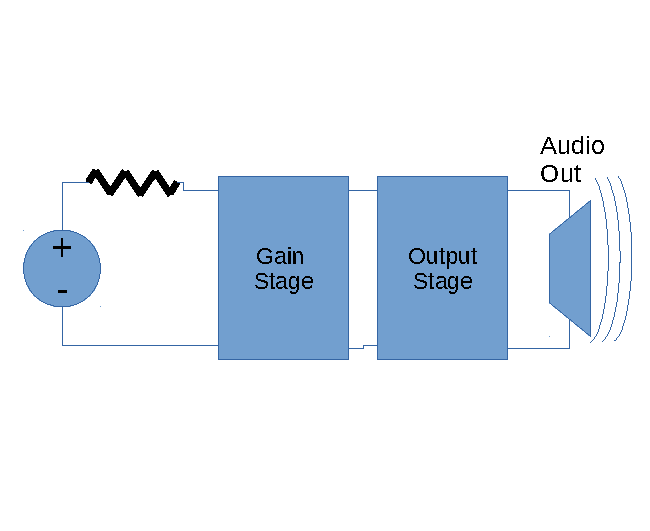
\includegraphics[width=0.65\linewidth]{doc/circ_enunciado.pdf}
	\caption{Assigned Circuit.}
	\label{fig:format}
\end{figure}

\begin{figure}[h!] \centering
	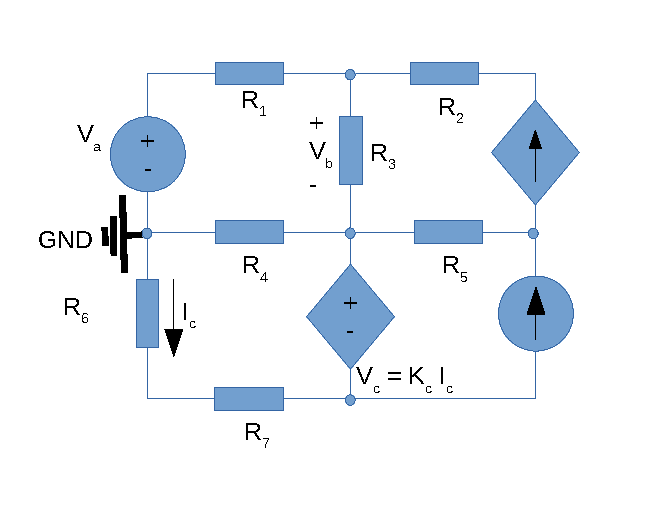
\includegraphics[width=0.6\linewidth]{circ.pdf}
	\caption{Chosen Circuit.}
	\label{fig:circuit}
\end{figure}

\emph{Note}: the diode in the voltage regulator is merely representative, as there are in fact 19 diodes in this subcircuit

